\typechapter{Shenyang JJ-2 and FT-2}

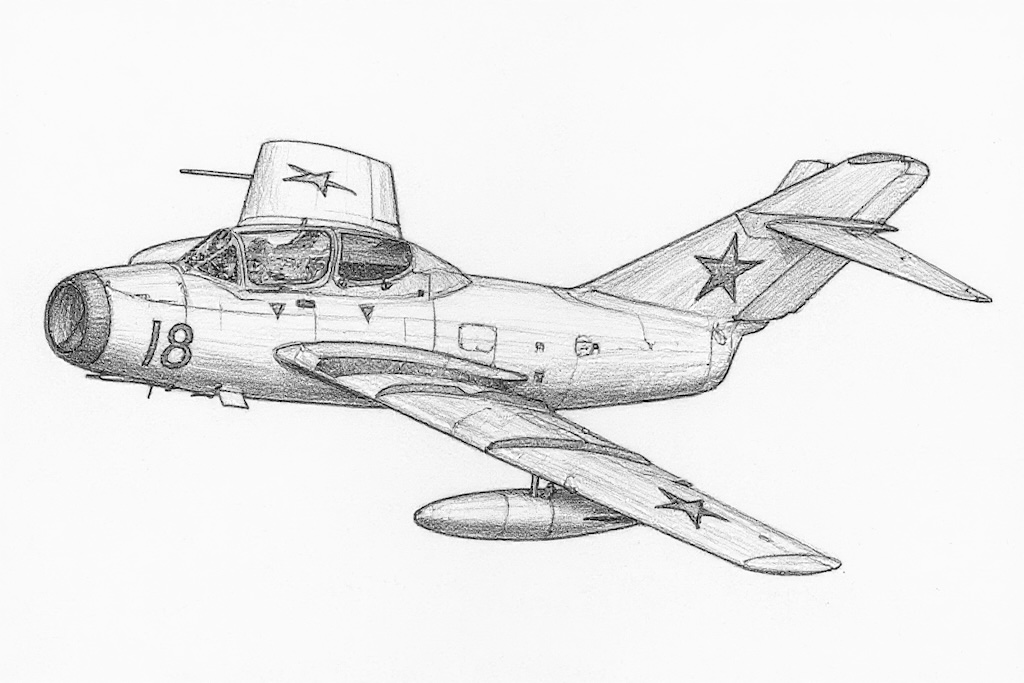
\includegraphics[width=\linewidth]{MiG-15UTI.jpg}

The Shenyang JJ-2 was a trainer, a licensed copy of the MiG-15UTI.

Many Soviet-built MiG-15bis fighters served in the PLAAF under the designation J-2, but unlike the JJ-2 the J-2 was not manufactured in China.

\section{Versions}

\subsection{JJ-2 and FT-2}

The Shenyang JJ-2 was a licensed copy of the MiG-15UTI trainer. The MiG-15UTI in turn was essentially a MiG-15 with a second cockpit and reduced armament. The FT-2 was the export version of the JJ-2. The NATO reporting name is Midget.

It was used extensively by the PLAAF and PLAN.

\section{Armament and Stores}

It is conceivable that the JJ-2 used the same stores as the MiG-15, especially 250L FTs.

\section{Combat}

The PLAN used the JJ-2 to attempt to intercept ROCAF overflights around 1960.

\section{ADCs}
\begin{adclist}
    \adcitem{Shenyang JJ-2}
    \adcitem{Shenyang FT-2}
\end{adclist}

\section{See Also}
\begin{typelist}
    \typeitem{Mikoyan-Gurevich MiG-15}
\end{typelist}

\section{Photo Credit}
\begin{itemize}\raggedright
        % I can't find a photo of a real JJ-2.
    \item \href{https://commons.wikimedia.org/wiki/File:Duxford_Air_Festival_2017_-_mig1_(34842016051).jpg}{MiG-15UTI}: wallycacsabre (CC-BY-2.0)
\end{itemize}
